% !TeX document-id = {e910d311-1b9f-412a-806f-acb4afe000c4}
% !TeX TXS-program:compile = txs:///pdflatex/[--shell-escape] | txs:///biber | txs:///pdflatex/[--shell-escape]
\documentclass[3p,times,a4paper,twocolumn,authoryear]{elsarticle} %authoryear

%% Fix so biblatex works instead of natbib
\makeatletter
\let\c@author\relax
\makeatother
\let\bibhang\relax
\let\citename\relax
\let\bibfont\relax
\let\Citeauthor\relax
\expandafter\let\csname ver@natbib.sty\endcsname\relax

%% Fix headers and footers
\makeatletter
\def\ps@pprintTitle{%
	\let\@oddhead\@empty
	\let\@evenhead\@empty
	\def\@oddfoot{\centerline{\thepage}}%
	\let\@evenfoot\@oddfoot}
\makeatother

%% Load some packages and stuff
%\usepackage[backend=biber,style=numeric, defernumbers=true, sorting=ynt,maxbibnames=4,maxcitenames=4]{biblatex}
%% Library and stuff
\usepackage[style=numeric,sortcites=true,sorting=ynt,backend=biber]{biblatex}
%% biblatex med apa-style. Det vivill ha
\DeclareLanguageMapping{american}{american-apa} %% Vi vill ha svensk apa
\bibliography{../bibliography/reference}

\usepackage[T1]{fontenc}
\usepackage[spanish]{babel}
\usepackage{pifont}
\usepackage{geometry}
\usepackage[svgnames]{xcolor}
\usepackage{graphicx}
\usepackage{sagetex}
\usepackage{minted}
\usepackage{float}
\usepackage{tkz-graph}
\usepackage{txfonts}
\usepackage{amsmath,amsthm}
\theoremstyle{definition}
\usepackage{bm}
\usepackage[colorlinks=true,urlcolor=blue,linkcolor=black,anchorcolor=black,citecolor=black]{hyperref}
\hypersetup{pdfinfo={
		Title={El teorema de los cuatro colores},
		Author={Grupo Nº6},
		Keywords={teorema de los cuatro colores, cadena de Kempe, grafos planares, coloración de mapas},
		Subject={Introducción a la matemática discreta},
		Producer={TeXstudio 2.12.8},
		Creator={pdfTeX Version 3.14159265 TeX Live 2018 Debian}
}}


\usepackage{etoolbox}
\AtBeginDocument{%
	%\patchcmd{<cmd>}{<search>}{<replace>}{<success>}{<failure>}
	%\patchcmd{\ps@pprintTitle}% <cmd>
	%{Preprint submitted}% <search>
	%{To be submitted}% <replace>
	%{}{}% <succes><failure>
	\patchcmd{\MaketitleBox}{\vspace*{-20pt}\fi}{\fi}{}{}%
	\patchcmd{\abstract}{Abstract}{Resumen}{}{}
	\patchcmd{\keyword}{Keywords}{Palabras clave}{}{}
}

%\makeatletter
%\patchcmd{\ps@pprintTitle}{\footnotesize\itshape
%	Preprint submitted to \ifx\@journal\@empty Elsevier
%	\else\@journal\fi\hfill\today}{\relax}{}{}
%\makeatother

\makeatletter
\def\printFirstPageNotes{%
	\iflongmktitle
	\let\columnwidth=\textwidth\fi
	\ifx\@tnotes\@empty\else\@tnotes\fi
	\ifx\@nonumnotes\@empty\else\@nonumnotes\fi
	\ifx\@cornotes\@empty\else\@cornotes\fi
	\ifx\@elseads\@empty\relax\else
	\let\thefootnote\relax
	\footnotetext{\ifnum\theead=1\relax
		\textit{Correo electrónico:\space}\else
		\textit{Correos electrónicos:\space}\fi
		\@elseads}\fi
	\ifx\@elsuads\@empty\relax\else
	\let\thefootnote\relax
	\footnotetext{\textit{Sitio web:\space}%
		\@elsuads}\fi
	\ifx\@fnotes\@empty\else\@fnotes\fi
	\iflongmktitle\if@twocolumn
	\let\columnwidth=\Columnwidth\fi\fi
}
\makeatother

%% `Elsevier LaTeX' style
%\bibliographystyle{elsarticle-num}
\renewcommand{\spanishcontentsname}{Tabla de contenidos}
\renewcommand{\spanishfigurename}{Fig.}
\renewcommand{\listingscaption}{Programa}
%\newcommand{\MVAt}{{\usefont{U}{mvs}{m}{n}\symbol{`@}}}
\newtheorem{definition}{Definición}
\newtheorem{example}{Ejemplo}
\newtheorem{theorem}{Teorema}

\graphicspath{{../images/}}

\usepackage{ecrc}

\volume{06}

\firstpage{10}

\runauth{Grupo N$^{\circ}6$}%C. Aznarán et al.

\jnltitlelogo{\large Annals of Discrete Mathematics FC-UNI}

\begin{document}

\begin{frontmatter}

\title{El teorema de los cuatro colores\tnoteref{t1}}
\tnotetext[t1]{This report is available on \href{https://github.com/carlosal1015/4colores}{GitHub}.}

%% Group authors per affiliation:
\author[1,3]{C.~Aznarán Laos}
\ead{caznaranl@uni.pe}

\author[1,3]{F.~Cruz Ordoñez\corref{mycorrespondingauthor}}
\ead{fransscruz18@gmail.com}

\author[2,3]{J.~Navío Torres\corref{mycorrespondingauthor}}
\ead{jnavio@uni.pe}
%\ead[url]{www.blogdeoromion.pe.hu}

%% or include affiliations in footnotes:
\author[1,3]{G.~Quiroz Gómez\corref{mycorrespondingauthor}}
\ead{ge\_qg\_25@hotmail.com}

\address[1]{Facultad de Ciencias - Escuela profesional de Ciencia de la Computación}
\address[2]{Facultad de Ciencias - Escuela profesional de Matemática}
\address[3]{Universidad Nacional de Ingeniería,	Av. Túpac Amaru 210, Rímac, Lima 25, Perú}
%\author[uni]{Álvaro I. Plasencia\corref{mycorrespondingauthor}}
%\cortext[mycorrespondingauthor]{Corresponding author}
%\ead{caznaranl@uni.pe}\fnref{fn1}
%\ead[url]{www.blogdeoromion.pe.hu}\fnref{fn1}
%\author[uni]{C. Aznarán\fnref{fn2}}
%\fntext[fn1]{First author partially supported by the Universidad Nacional de Ingeniería project.}
%\fntext[fn2]{Second author partially supported by the Undergraduate Mathematics Group P156250.}
%
\begin{abstract}
En este reporte, nosotros repasaremos las definiciones acerca de los grafos planares, grafos duales, número cromático y polinomio cromático. Además, nosotros mostraremos la interrelación entre este tipo de grafos. Al haber presentado las definiciones establecidas para los grafos duales, se buscará una representación analógica para los mapas conexos. También se dará una introducción a las cadenas de Kempe y se dará una prueba completa del contraejemplo del grafo de Errera el cual está presentado en \cite{birkhoff}.
\\[0.2cm]
%In this paper, we will review the definitions about the hyperbolic functions, trigonometric functions and deduce their inverse functions in terms of logarithms and exponentials introducing complex numbers.
%Hence, we will show the mathematical interrelation between this types of functions.
%Having already present the established definitions for the hyperbolic functions will look for an analog representation for the trigonometric functions.% We will also give an introduction to inverse hyperbolic functions.
\textcopyright \hspace{.1cm}Science Department National University of Engineering Publishers Inc. All rights reserved. 
\end{abstract}

\begin{keyword}
teorema de los cuatro colores \sep cadena de Kempe\sep grafos planares\sep coloración de mapas
\end{keyword}

\end{frontmatter}

\tableofcontents

\section{Introducción}
Si $G$ es un grafo sin lazos, entonces $G$ es \textbf{$\bm{k}$-coloreable} si podemos asignar uno de $k$ colores a cada vértices de manera que vértices adyacentes tengas diferentes colores. Si $G$ es $k$-coloreable, pero no $(k-1)$- coloreable, diremos que $G$ es \textbf{$\bm{k}$-cromático}, o que el \textbf{número cromático} de $G$ es $k$, y lo denotamos por $\chi(G)=k$. Por ejemplo, la Figura~\ref{fig:1.1} muestra un grafo para el cual $\chi(G)=4$; los colores son dentados por las letras griegas. Es por lo tanto $k$-coloreable si $k>4$. Deberíamos asumir que todos los grafos aquí son simples, ya que los bordes múltiples son irrelevantes para nuestra discusión. También asumiremos que están conectados.

Es claro que $\chi(K_n)=n$, y así, existen grafos con un número cromático grande y arbitrario. En el otro extremo de la escala, $\chi(G)=1$ si y solo si $G$ es el grafo nulo, y $\chi(G)=2$ si y solo si $G$ es un grafo bipartito no nulo. Note que cualquier árbol es $2$-coloreable, así como cualquier ciclo con un número par de vér

\begin{figure}[H]
\centering
\scalebox{0.6}{\begin{tikzpicture}
	\SetGraphUnit{4}
	\GraphInit[vstyle=Classic]
	%\SetVertexNoLabel
	\Vertex[L={\LARGE$\alpha$}, Lpos=180]{a}
	\EA[L={\LARGE$\gamma$}](a){b}
	\NOEA[L={\LARGE$\beta$},Lpos=90](b){c}
	\SOEA[L={\LARGE$\delta$}, Lpos=-90](b){d}
	\EA[unit=7, L={\LARGE$\alpha$}](b){e}
	\Edges(d,a,b,c,e,d,c,c,a,b,d)
\end{tikzpicture}}
\caption{Grafo $G$}\label{fig:1.1}
\end{figure}

\begin{definition}[Grafo planar]
Un dibujo de un grafo $G=(V,E)$ es una aplicación que a cada vértice $v$ del grafo $G$ le asigna un punto $b(v)$ del plano, y a cada rama $e=\{v,v^{\prime}\}\in E$, le asigna un arco $\alpha(e)$ del plano con $b(v)$ y $b(v^{\prime})$como puntos finales. Suponemos que la aplicación $b$ es inyectiva (vértices diferentes tienen asignados distintos puntos del plano), y un punto de la forma $b(v)$ no está en ninguno de los arcos $\alpha(e)$ excepto si es un punto final de este arco. Un grafo junto con alguno de sus dibujos se llama grafo topológico.
\end{definition}

\begin{theorem}[Teorema de Kuratowski]
Un grafo $G$ es planar si y solo si no tiene ningún subgrafo isomorfo a una subdivisión de $K_{3,3}$ o una subdivisión de $K_5$.
\end{theorem}

\begin{definition}[Mapa conexo]
Un mapa es conexo\footnote{De una sola pieza.} y cada una de sus regiones también es conexa.
\end{definition}

\begin{definition}[Número cromático] 
Sea $G=(V,E)$ un grafo y sea $k$ un número natural. Una aplicación $c\colon V\to \{1,2,\ldots k\}$ se llama \emph{\color{DarkBlue}coloración del grafo} $G$ si $c(x)\neq c(y)$ se cumple para cada rama $\{x,y\}\in E$. \linebreak El \emph{\color{DarkBlue}número cromático} de $G$, denotado por $\chi(G)$, es el \emph{\color{red}mínimo valor} de $k$ para el cual existe una coloración $c\colon V(G)\to\{1,2\ldots,k\}$.
\end{definition}

\begin{definition}[Grafo Dual]
Sea $G=(V,E)$ un grafo planar con un dibujo planar fijo. Denotamos por $\mathcal{F}$ el conjunto de caras de $G$. Definimos un grafo, con posibles lazos y ramas múltiples, como $(\mathcal{F},E,\varepsilon)$, donde $\varepsilon$ se define como $\varepsilon(e)=\{F_i,F_j\}$ siempre que la rama $e$ sea una frontera común de las caras $F_i$ y $F_j$.

Este grafo $\left(\mathcal{F},E,\varepsilon\right)$ se le llama el dual de $G$ y se denota por $G^{\ast}$.	
\end{definition}

\begin{example}[Grafos Duales]
Para construir una gráfica dual de un grafo plano $G$ se debe colocar un vértice dentro de cada región de $G$ e incluir la región infinita de $G$. Para cada arista compartida por las $2$ regiones, se debe dibujar una arista que conecte a los vértices dentro de estas regiones y para cada arista que se recorre $2$ veces en el camino cerrado alrededor de las aristas de una región se dibuja un lazo en el vértice de la región. 
\end{example}

\begin{figure}[H]
\centering
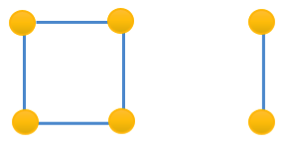
\includegraphics[width=3cm]{example1}
\caption{Grafo $G$.}
\end{figure}

\begin{figure}[H]
	\centering
	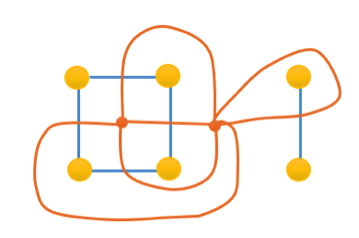
\includegraphics[width=3cm]{example2}
	\caption{Grafo $G$.}
\end{figure}

\begin{figure}[H]
	\centering
	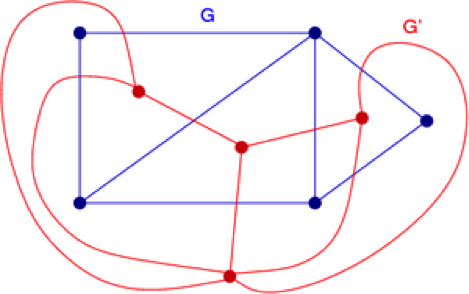
\includegraphics[width=3cm]{example3}
	\caption{Grafo $G$.}
\end{figure}
\subsection{El problema de los cuatro colores}

\subsection{Algunas fechas importantes}

\section{El ``camino'' hacia la demostración}

\subsection{La formulación de la conjetura}

\subsection{La primera ``demostración'': las cadenas de Kempe}

\begin{definition}[Polinomio cromático]
Sea $G=(V,E)$ un grafo planar y $P(G,k)$ el número de vértices coloreados.
El polinomio cromático cuenta el número de maneras que puede ser coloreado un grafo usando no más de número dado de colores.
\end{definition}

\begin{definition}[Cadenas de Kempe]
Suponga que un mapa $M$ es coloreado por los colores $a, b, c$ y $d$, seleccione un par de ellos, como $a$ y $b$. Considere cualquier región coloreada en uno de esos pares de colores juntos con todas las regiones de esos colores, adyacente o conexa por un conjunto de regiones en los dos colores. Tal conjunto de regiones será llamado una \emph{cadena} $a,b$. Obviamente, la misma cadena $a,b$ es definida por cualquier región en la cadena.

Una propiedad fundamental de la cadena es que si los dos colores sobre las regiones de una cadena simple, o de cualquier conjunto de esas cadenas de los mismos colores, todas intercambiadas, una nueva coloración de mapas resulta
\end{definition}

\begin{definition}[Cadena de Kempe]
Sea $G$ un grafo planar cuyos vértices han sido coloreados apropiadamente y suponga $v\in V(G)$ es coloreado $C_1$. Definimos la \emph{cadena de Kempe} $C_1C_2$ que contiene a $v$ para ser el componente conexa maximal de $G$ que

\begin{enumerate}%[label=\arabic*]
	\item Contiene a $v$, y
	\item Contenga solo vértices que son coloreados con elementos desde $(C_1C_2)$.
	\end{enumerate}
\end{definition}

\subsection{Heawood y el error fatal de \citeauthor{kempe}}

\subsection{Idea clave: la reducibilidad de mapas de \citeauthor{birkhoff}}

\subsection{El método de descarga de \citeauthor{appel}}

\section{Aplicaciones}

\subsection{El juego Hex}

\section{Conclusiones}

\subsection{Importancia del teorema para los matemáticos}

\section*{Agradecimientos}

The authors want to thank the Universidad Nacional de Ingeniería and the Undergraduate Mathematics Group for their hospitality during the visits while preparing this paper.

The authors would like to thank professor Johny Valverde for many valuable and constructive suggestions, that have helped to improve the paper.

\nocite{*}
\printbibliography[title={Referencias}]
\end{document}
https://www.overleaf.com/17245402qmwcfgzsxdrd#/65670813/
ANTECEDENTES
• 1852: Francis Guthrie plantea el problema a su hermano Frederick y éste a Augustus de Morgan.
• 1878: Arthur Cayley publica el enunciado de la conjetura.
• 1879: Sir Alfred Bray Kempe publica su demostración.
• 1890: Percy Heawood descubre un error insalvable en la prueba dada por Kempe.
• 1913: George Birkhoff introduce la noción de configuración reducible.
• 1960: Se introduce el llamado método de descarga.
• 1969: Avances de Heinrich Heesch en reducibilidad y obtención de conjuntos inevitables de configuraciones.
• 1976: Ken Appel y Wolfgang Haken prueban con ayuda de un ordenador que sus 1.482 configuraciones son reducibles (50 días de cálculo).
• 1996: N. Robertson, D.P. Sanders, P. Seymour y R. Thomas mejoran la demostración con ayuda de ordenador (sólo 633 configuraciones) y automatizan la prueba de la inevitabilidad.
• 2000: Ashay Dharwadker da otra prueba del teorema de los 4 colores, no basada en ideas previas, utilizando teoría de grupos, teoría de sistemas de Steiner y correspondencias de Hall
• 2004: Ibrahim Cahit, dice haber demostrado la conjetura, usando el nuevo concepto de cadenas espirales, sin ordenador.
Línea de tiempo